\chapter{Cinemática}
A Física como ciência é muito vasta e requer subdivisões de estudo, uma das grandes areas que estuda o movimento em condições específicas é a cinemática. 

A cinemática estuda o movimento dos corpos sem se preocupar com as causas que o produzem, ou seja, a cinemática descreve como os corpos se movem, enquanto a dinâmica estuda por que os corpos se movem.

\section{Conceitos Fundamentais}

Antes de estudarmos o movimento, precisamos entender alguns conceitos básicos, como referencial, ponto material, corpo extenso e trajetória.

\subsection{Referencial e Sistemas de Coordenadas}

O \textbf{referencial} é o corpo ou lugar a partir do qual observamos os fenômenos. Para quantificar essa observação, utilizamos um \textbf{sistema de coordenadas}.

\subsubsection{Sistema de Coordenadas e a Origem}
O sistema de coordenadas \ref{fig:sistemas_coordenadas} permite localizar o móvel no espaço. Todo sistema possui uma \textbf{origem} (Ponto Zero), que é o ponto de referência para a contagem das posições ($s$).

% --- Exemplo de Sistema Unidimensional ---
\begin{figure}[htbp]
    \centering
    % --- Subfigura A: Unidimensional ---
    \begin{subfigure}[b]{0.45\textwidth}
        \centering
        \begin{tikzpicture}[>=stealth, scale=0.8]
            \draw[->, thick] (-2.5,0) -- (2.5,0) node[right] {$s$};
            \foreach \x in {-2,-1,0,1,2}
                \draw (\x, 0.1) -- (\x, -0.1) node[below] {\scriptsize \x};
            \filldraw[azul] (0,0) circle (2pt) node[above=2pt] {\scriptsize $O$};
            \filldraw[vermelho] (1.5,0) circle (2pt);
        \end{tikzpicture}
        \caption{Sistema Unidimensional (Reta)}
        \label{fig:coord_unidim}
    \end{subfigure}
    \hfill % Espaçamento entre as figuras
    % --- Subfigura B: Bidimensional ---
    \begin{subfigure}[b]{0.45\textwidth}
        \centering
        \begin{tikzpicture}[>=stealth, scale=0.6]
            \draw[->, thick] (-1,0) -- (3,0) node[right] {$x$};
            \draw[->, thick] (0,-1) -- (0,3) node[above] {$y$};
            \draw[help lines, dashed] (0,0) grid (2,2);
            \filldraw[azul] (0,0) circle (3pt) node[below left] {\scriptsize $O$};
            \filldraw[vermelho] (2,2) circle (3pt) node[above right] {\scriptsize $P(2,2)$};
        \end{tikzpicture}
        \caption{Sistema Bidimensional (Plano)}
        \label{fig:coord_bidim}
    \end{subfigure}

    \vspace{0.3cm}
    \caption{Representação visual dos sistemas de coordenadas e suas respectivas origens ($O$).}
    \label{fig:sistemas_coordenadas}
\end{figure}

\begin{itemize}
    \item \textbf{Movimento:} Variação da posição ao longo do tempo em relação ao referencial.
    \item \textbf{Repouso:} Posição sem alteração ao longo do tempo de acordo com o referencial adotado.
\end{itemize}

% Exemplo de relatividade do movimento
\begin{figure}[htbp]
    \centering
    \includegraphics[width=0.8\textwidth]{figuras/fig-01.png}
    \caption[Movimento relativo no ônibus]{Ilustração do movimento relativo de uma esfera: Na figura superior, nota-se um passageiro observando o movimento vertical de uma esfera. Na figura inferior, nota-se umm observador externo visualizando uma trajetória parabólica da mesma esfera.}
    \label{fig:movimento_relativo}
\end{figure}

Qualquer corpo móvel ou fixo pode ser escolhido como referencial, desde que sua posição seja conhecida. O sistema de coordenadas é definido após estabelecer a métrica que frequentemente assume valores dentro do SI.

\subsubsection{Exemplo Prático}
Considere uma rodovia: o quilômetro zero é a \textbf{origem}. Se um carro está parado no KM 20, ele está em repouso em relação à rodovia, mas em movimento em relação ao Sol \parencite{halliday2012}.

\subsection{Ponto Material e Corpo Extenso}

A classificação de um móvel depende da escala do fenômeno observado.

\begin{itemize}
    \item \textbf{Ponto Material:} Suas dimensões são desprezíveis em relação ao fenômeno. Ex: Um planeta orbitando o Sol.
    \item \textbf{Corpo Extenso:} Suas dimensões são relevantes e influenciam no estudo. Ex: Um planeta sendo estudado quanto à sua rotação e inclinação do eixo.
\end{itemize}

% Exemplo de ponto material vs corpo extenso
\begin{figure}[htbp]
    \centering
    \includegraphics[width=0.6\textwidth]{figuras/fig-02.png}
    \caption[Movimento relativo no ônibus]{A figura demonstra a diferença entre um ponto material e um corpo extenso. À esquerda, uma pessoa sob uma superfície muito extensa. A direita, uma pessoa em uma superfície pequena, onde suas dimensões são relevantes.}
    \label{fig:corpo_ponto}
\end{figure}

\subsubsection{Critério de Diferenciação}
Para diferenciar, comparamos o tamanho do objeto ($L$) com a distância percorrida ($D$):
\begin{itemize}
    \item Se $L \ll D$ (muito menor), temos um \textbf{ponto material}.
    \item Se $L \approx D$ (comparável), temos um \textbf{corpo extenso}.
\end{itemize}

\subsection{Trajetória}
É o lugar geométrico das posições sucessivas do móvel. Sua forma depende do referencial.

\section{Tipos de Movimento}
\begin{itemize}
    \item \textbf{Progressivo:} $v > 0$ (segue a orientação da via).
    \item \textbf{Retrógrado:} $v < 0$ (contra a orientação da via).
\end{itemize}

\begin{figure}[htbp]
    \centering
    % --- CASO 1: MOVIMENTO PROGRESSIVO ---
    \begin{subfigure}[b]{0.48\textwidth}
        \centering
        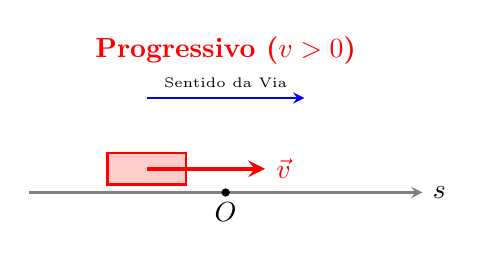
\begin{tikzpicture}[>=stealth]
            % Eixo da trajetória
            \draw[->, thick, gray] (-2.5,0) -- (2.5,0) node[right, black] {$s$};
            \fill (0,0) circle (1.5pt) node[below] {$O$};
            
            % Sentido Positivo da Via
            \draw[->, blue, thick] (-1, 1.2) -- (1, 1.2) node[midway, above, black] {\tiny Sentido da Via};
            
            % O Móvel (Progressivo)
            \draw[fill=red!20, draw=red, thick] (-1.5, 0.1) rectangle (-0.5, 0.5);
            \draw[->, red, ultra thick] (-1, 0.3) -- (0.5, 0.3) node[right] {$\vec{v}$};
            
            \node[red, font=\bfseries] at (0, 1.8) {Progressivo ($v > 0$)};
        \end{tikzpicture}
        \caption{Mesmo sentido da trajetória.}
    \end{subfigure}
    \hfill % Este comando joga o próximo desenho para a outra ponta
    % --- CASO 2: MOVIMENTO RETRÓGRADO ---
    \begin{subfigure}[b]{0.48\textwidth}
        \centering
        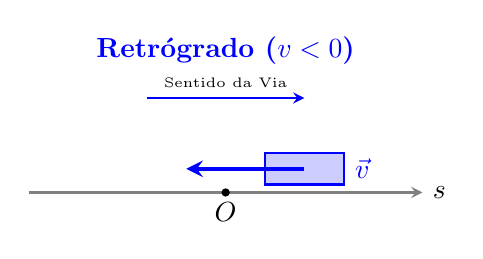
\begin{tikzpicture}[>=stealth]
            % Eixo da trajetória
            \draw[->, thick, gray] (-2.5,0) -- (2.5,0) node[right, black] {$s$};
            \fill (0,0) circle (1.5pt) node[below] {$O$};
            
            % Sentido Positivo da Via
            \draw[->, blue, thick] (-1, 1.2) -- (1, 1.2) node[midway, above, black] {\tiny Sentido da Via};
            
            % O Móvel (Retrógrado)
            \draw[fill=blue!20, draw=blue, thick] (0.5, 0.1) rectangle (1.5, 0.5);
            \draw[<-, blue, ultra thick] (-0.5, 0.3) -- (1, 0.3) node[right, xshift=0.5cm] {$\vec{v}$};
            
            \node[blue, font=\bfseries] at (0, 1.8) {Retrógrado ($v < 0$)};
        \end{tikzpicture}
        \caption{Sentido oposto à trajetória.}
    \end{subfigure}

    \vspace{0.5cm}
    \caption{Classificação do sentido do movimento em relação à orientação da trajetória.}
    \label{fig:progressivo_retrogrado}
\end{figure}

\section{Velocidade}
Mensura a taxa de variação da posição em relação ao tempo. Pode ser classificada em:
\begin{itemize}
    \item \textbf{Velocidade Escalar Média:} Grandeza escalar que indica a rapidez média de um móvel.
    \item \textbf{Velocidade Instantânea:} Grandeza vetorial que indica a velocidade em um instante específico.
\end{itemize}

\subsection{Velocidade Instantânea}
A velocidade instantânea é a taxa de variação da posição num intervalo de tempo próximo a zero. É mensurado com o velocímetro do veículo. Podemos entender como um limite da velocidade média quando o intervalo de tempo tende a zero. 

\subsection{Velocidade Escalar Média}
A velocidade escalar média descreve a velocidade em que se deve ter, de maneira fixa, para percorrer uma dada distância naquele tempo. Diferente da velocidade instantânea, essa velocidade descreve todo um trajeto. 
A velocidade média pode ser determinada pela razão entre a distância percorrida ($\Delta s$) com o intervalo de tempo gasto ($\Delta t$), como podemos ver na equação \ref{eq:velocidade_media}.
\begin{equation}
    v_m = \frac{\Delta s}{\Delta t} \label{eq:velocidade_media}
\end{equation}
Com:
\begin{equation*}
    \begin{aligned}
        \Delta s = s_f - s_i & \xmapsto{\hspace{1.5cm}} \text{Variação da posição (Deslocamento)} \\
        \Delta t = t_f - t_i & \xmapsto{\hspace{1.5cm}} \text{Variação do tempo (Intervalo)} \\
        v_m & \xmapsto{\hspace{1.5cm}} \text{Velocidade Escalar Média}
    \end{aligned}
\end{equation*}